%% BioMed_Central_Tex_Template_v1.06
%%                                      %
%  bmc_article.tex            ver: 1.06 %
%                                       %

%%IMPORTANT: do not delete the first line of this template
%%It must be present to enable the BMC Submission system to
%%recognise this template!!


%%% Alternative Method for Adding supplemental figures
% http://bytesizebio.net/2013/03/11/adding-supplementary-tables-and-figures-in-latex/
%%%%%%%%%%%%%%%%%%%%%%%%%%%%%%%%%%%%%%%%%
%%                                     %%
%%  LaTeX template for BioMed Central  %%
%%     journal article submissions     %%
%%                                     %%
%%          <8 June 2012>              %%
%%                                     %%
%%                                     %%
%%%%%%%%%%%%%%%%%%%%%%%%%%%%%%%%%%%%%%%%%


%%%%%%%%%%%%%%%%%%%%%%%%%%%%%%%%%%%%%%%%%%%%%%%%%%%%%%%%%%%%%%%%%%%%%
%%                                                                 %%
%% For instructions on how to fill out this Tex template           %%
%% document please refer to Readme.html and the instructions for   %%
%% authors page on the biomed central website                      %%https://www.overleaf.com/1872464598fyjkfhmssdhj
%% http://www.biomedcentral.com/info/authors/                      %%
%%                                                                 %%
%% Please do not use \input{...} to include other tex files.       %%
%% Submit your LaTeX manuscript as one .tex document.              %%
%%                                                                 %%
%% All additional figures and files should be attached             %%
%% separately and not embedded in the \TeX\ document itself.       %%
%%                                                                 %%
%% BioMed Central currently use the MikTex distribution of         %%
%% TeX for Windows) of TeX and LaTeX.  This is available from      %%
%% http://www.miktex.org                                           %%
%%                                                                 %%
%%%%%%%%%%%%%%%%%%%%%%%%%%%%%%%%%%%%%%%%%%%%%%%%%%%%%%%%%%%%%%%%%%%%%

%%% additional documentclass options:
%  [doublespacing]
%  [linenumbers]   - put the line numbers on margins

%%% loading packages, author definitions

% \documentclass[twocolumn]{bmcart}% uncomment this for twocolumn layout and comment line below
\documentclass[linenumbers]{bmcart}

%%% Load packages
\usepackage{amsthm,amsmath}
%\RequirePackage{natbib}
%\RequirePackage[authoryear]{natbib}% uncomment this for author-year bibliography
\RequirePackage{hyperref}
\usepackage[utf8]{inputenc} %unicode support
% \usepackage[applemac]{inputenc} %applemac support if unicode package fails
%\usepackage[latin1]{inputenc} %UNIX support if unicode package fails
\usepackage{lmodern}
\usepackage{booktabs,longtable,multirow}
\usepackage{threeparttable}
\usepackage{pdflscape}
\usepackage{makecell}

%%%%%%%%%%%%%%%%%%%%%%%%%%%%%%%%%%%%%%%%%%%%%%%%%
%%                                             %%
%%  If you wish to display your graphics for   %%
%%  your own use using includegraphic or       %%
%%  includegraphics, then comment out the      %%
%%  following two lines of code.               %%
%%  NB: These line *must* be included when     %%
%%  submitting to BMC.                         %%
%%  All figure files must be submitted as      %%
%%  separate graphics through the BMC          %%
%%  submission process, not included in the    %%
%%  submitted article.                         %%
%%                                             %%
%%%%%%%%%%%%%%%%%%%%%%%%%%%%%%%%%%%%%%%%%%%%%%%%%

%%%% Remove comments prior to re-submission
\def\includegraphic{}
\def\includegraphics{}



%%% Put your definitions there:
\startlocaldefs
\endlocaldefs


%%% Begin ...
\begin{document}

%%% Start of article front matter
\begin{frontmatter}

\begin{fmbox}
\dochead{Research}

%%%%%%%%%%%%%%%%%%%%%%%%%%%%%%%%%%%%%%%%%%%%%%
%%                                          %%
%% Enter the title of your article here     %%
%%                                          %%
%%%%%%%%%%%%%%%%%%%%%%%%%%%%%%%%%%%%%%%%%%%%%%

\title{A framework for assessing 16S rRNA marker-gene survey data analysis methods using mixtures.}

%%%%%%%%%%%%%%%%%%%%%%%%%%%%%%%%%%%%%%%%%%%%%%
%%                                          %%
%% Enter the authors here                   %%
%%                                          %%
%% Specify information, if available,       %%
%% in the form:                             %%
%%   <key>={<id1>,<id2>}                    %%
%%   <key>=                                 %%
%% Comment or delete the keys which are     %%
%% not used. Repeat \author command as much %%
%% as required.                             %%
%%                                          %%
%%%%%%%%%%%%%%%%%%%%%%%%%%%%%%%%%%%%%%%%%%%%%%

\author[
   addressref={aff1,aff2,aff3},                   % id's of addresses, e.g. {aff1,aff2}
   corref={aff1},                       % id of corresponding address, if any
   % noteref={n1},                        % id's of article notes, if any
   email={nolson@nist.gov}   % email address
]{\inits{ND}\fnm{Nathan D.} \snm{Olson}}
\author[
   addressref={aff2,aff3},
   email={smuthiah@umiacs.umd.edu}
]{\inits{MS}\fnm{M. Senthil} \snm{Kumar}}
\author[
   addressref={aff4},
   email={sli1@epi.umaryland.edu}
]{\inits{S}\fnm{Shan} \snm{Li}}
\author[
   addressref={aff2,aff3},
   email={dbraccia@umd.edu}
]{\inits{DJB}\fnm{Domenick J.} \snm{Braccia}}
\author[
   addressref={aff5},
   email={shao4@jhu.edu}
]{\inits{S}\fnm{Stephanie} \snm{Hao}}
\author[
   addressref={aff5},
   email={wtimp@jhu.edu}
]{\inits{W}\fnm{Winston} \snm{Timp}}
\author[
   addressref={aff6},
   email={msalit@stanford.edu}
]{\inits{ML}\fnm{Marc L.} \snm{Salit}}
\author[
   addressref={aff4},
   email={cstine@som.umaryland.edu}
]{\inits{OC}\fnm{O. Colin} \snm{Stine}}
\author[
   addressref={aff2,aff3,aff7},
   email={hcorrada@umiacs.umd.edu}
]{\inits{H}\fnm{Hector} \snm{Corrada Bravo}}


%%%%%%%%%%%%%%%%%%%%%%%%%%%%%%%%%%%%%%%%%%%%%%
%%                                          %%
%% Enter the authors' addresses here        %%
%%                                          %%
%% Repeat \address commands as much as      %%
%% required.                                %%
%%                                          %%
%%%%%%%%%%%%%%%%%%%%%%%%%%%%%%%%%%%%%%%%%%%%%%

\address[id=aff1]{%                           % unique id
  \orgname{Biosystems and Biomaterials Division, National Institute of Standards and Technology},
  \street{100 Bureau Dr.},
  \city{Gaithersburg, Maryland},
  \postcode{20899}
  \cny{USA}
}
\address[id=aff2]{%
  \orgname{Center for Bioinformatics and Computational Biology, University of Maryland, College Park},
  \street{8314 Paint Branch Dr.}
  \city{College Park, Maryland},
  \postcode{20742}
  \cny{USA}
}
\address[id=aff3]{%
  \orgname{University of Maryland Institute of Advanced Computer Studies, University of Maryland, College Park},
  \street{8223 Paint Branch Dr.}
  \city{College Park, Maryland},
  \postcode{20742}
  \cny{USA}
}
\address[id=aff4]{%
  \orgname{Department of Epidemiology and Public Health, University of Maryland School of Medicine},
  \street{655 W. Baltimore Street},
  \city{Baltimore, Maryland},
  \postcode{21201}
  \cny{USA}
}
\address[id=aff5]{%
  \orgname{Department of Biomedical Engineering, Johns Hopkins University},
  \street{720 Rutland Ave.},
  \city{Baltimore, Maryland},
  \postcode{21205}
  \cny{USA}
}
\address[id=aff6]{%
  \orgname{Joint Initiative for Metrology in Biology},
  \street{443 Via Ortega},
  \city{Stanford, CA},
  \postcode{94305}
  \cny{USA}
}
\address[id=aff7]{%
  \orgname{Department of Computer Science, University of Maryland, College Park},
  \street{8223 Paint Branch Dr.}
  \city{College Park, Maryland},
  \postcode{20742}
  \cny{USA}
}

%%%%%%%%%%%%%%%%%%%%%%%%%%%%%%%%%%%%%%%%%%%%%%
%%                                          %%
%% Enter short notes here                   %%
%%                                          %%
%% Short notes will be after addresses      %%
%% on first page.                           %%
%%                                          %%
%%%%%%%%%%%%%%%%%%%%%%%%%%%%%%%%%%%%%%%%%%%%%%

\begin{artnotes}
%\note{Sample of title note}     % note to the article
% \note[id=n1]{Equal contributor} % note, connected to author
\end{artnotes}

\end{fmbox}% comment this for two column layout

%%%%%%%%%%%%%%%%%%%%%%%%%%%%%%%%%%%%%%%%%%%%%%
%%                                          %%
%% The Abstract begins here                 %%
%%                                          %%
%% Please refer to the Instructions for     %%
%% authors on http://www.biomedcentral.com  %%
%% and include the section headings         %%
%% accordingly for your article type.       %%
%%                                          %%
%%%%%%%%%%%%%%%%%%%%%%%%%%%%%%%%%%%%%%%%%%%%%%

\begin{abstractbox}

\begin{abstract} % abstract

\parttitle{Background}
Analysis of 16S rRNA marker-gene surveys may be performed by a variety of bioinformatic pipelines and downstream analysis methods. However, appropriate assessment datasets and statistics are needed as there is limited guidance to decide between available analysis methods. Mixtures of environmental samples are useful for assessment as they provide values calculated from measurements of the unmixed samples and the mixture design that can be compared to values recovered by each bioinformatic method.
While experiments mixing complex samples have been used to assess other sequencing methods such as RNAseq, they have yet to be used to assess 16S rRNA sequencing.


\parttitle{Results}
We developed an assessment framework for 16S rRNA sequencing analysis methods 
based on a two-sample titration mixture dataset and metrics to evaluate OTU count table characteristics. 
Our qualitative assessment evaluates feature presence/absence exploiting features only present in unmixed samples or titrations by testing if random sampling can explain their observed relative abundance.
Our quantitative assessment evaluates how well relative and differential abundance values agree with values expected from the mixture design.
We evaluated count tables generated by three commonly used bioinformatic pipelines as demonstration:
i) DADA2 a sequence inference method, ii) Mothur a \textit{de novo} clustering method, and iii) QIIME which uses open-reference clustering.
Qualitative assessment indicated that the majority of Mothur and QIIME features specific to unmixed samples or titrations were explained by random sampling alone but not DADA2 features.
When combined with assessments of count table sparsity, these results indicate that DADA2 has a higher false negative rate whereas Mothur and QIIME have higher false positive rates.
Quantitative assessment indicated that, overall, observed relative abundance and differential abundance values were consistent with expected values for all three pipelines. We also identified subsets of features measured with high error by all pipelines evaluated. We could not identify the source of bias in these poor performing features based on previously studied sources of bias, indicating that further analysis of potentially unknown and unaccounted for biases is warranted. 

\parttitle{Conclusions}
We developed a novel framework for assessing 16S rRNA marker-gene survey analysis methods based on mixture experiments.
To demonstrate the assessment framework we evaluated count tables generated using three bioinformatic pipelines.
The assessment framework developed for this study will serve as a valuable community resource for assessing 16S rRNA marker-gene survey bioinformatic methods.

\end{abstract}

%%%%%%%%%%%%%%%%%%%%%%%%%%%%%%%%%%%%%%%%%%%%%%
%%                                          %%
%% The keywords begin here                  %%
%%                                          %%
%% Put each keyword in separate \kwd{}.     %%
%%                                          %%
%%%%%%%%%%%%%%%%%%%%%%%%%%%%%%%%%%%%%%%%%%%%%%

\begin{keyword}
\kwd{16S rRNA gene}
\kwd{assessment}
\kwd{bioinformatic pipeline}
\kwd{normalization}
\kwd{differential abundance}
\end{keyword}

% MSC classifications codes, if any
%\begin{keyword}[class=AMS]
%\kwd[Primary ]{}
%\kwd{}
%\kwd[; secondary ]{}
%\end{keyword}

\end{abstractbox}
%
%\end{fmbox}% uncomment this for twcolumn layout

\end{frontmatter}

%%%%%%%%%%%%%%%%%%%%%%%%%%%%%%%%%%%%%%%%%%%%%%
%%                                          %%
%% The Main Body begins here                %%
%%                                          %%
%% Please refer to the instructions for     %%
%% authors on:                              %%
%% http://www.biomedcentral.com/info/authors%%
%% and include the section headings         %%
%% accordingly for your article type.       %%
%%                                          %%
%% See the Results and Discussion section   %%
%% for details on how to create sub-sections%%
%%                                          %%
%% use \cite{...} to cite references        %%
%%  \cite{koon} and                         %%
%%  \cite{oreg,khar,zvai,xjon,schn,pond}    %%
%%  \nocite{smith,marg,hunn,advi,koha,mouse}%%
%%                                          %%
%%%%%%%%%%%%%%%%%%%%%%%%%%%%%%%%%%%%%%%%%%%%%%


\section*{Background}

Targeted sequencing of the 16S rRNA gene is commonly used to characterize
microbial communities. The 16S rRNA marker-gene-survey
measurement process includes molecular steps to selectively target and sequence the 16S rRNA
gene from prokaryotic organisms within a sample and
computational steps \cite{Goodrich2014} computational steps
convert the raw sequence data into a count table of feature relative abundance values
\cite{Goodrich2014}. Both molecular and computational measurement
processes contribute to the overall measurement bias and dispersion
\cite{Amore2016, Goodrich2014, brooks2015truth}. The need for datasets characterizing complex microbial communities with
some degree ``ground truth'' has emerged in order to properly characterize the accuracy of the 16S rRNA
marker-gene-survey measurement process.

Diverse bioinformatic pipelines used to generate count tables produce data with diverse characteristics.
For example the commonly used QIIME, Mothur, and
DADA2 pipelines produce feature sets and count tables with different characteristics. 
Mothur uses \emph{de novo} clustering for feature
inference \cite{westcott2017opticlust, schloss2009introducing}.
Pairwise distances used in clustering are calculated from a multiple
sequence alignment. Quality filtered paired-end reads are merged
into contigs, then aligned to a reference multiple
sequence alignment, followed by the removal of uninformative positions.
As a result the feature set representative sequences are shorter than the input amplicons. 
For the QIIME open-reference clustering pipeline merged paired-end reads are first assigned to reference cluster
centers \cite{Rideout2014, Caporaso2010}. 
Next, unassigned reads are clustered \emph{de novo}. 
Unlike Mothur, the QIIME pipeline clustering method uses pairwise sequence distances calculated from pairwise sequence alignments. 
As a result, the QIIME pairwise distances are calculated using the full amplicon sequence, 
whereas Mothur pairwise distances are calculated using multiple sequence alignment with only informative positions.
The DADA2 pipeline uses a probability model and maximization expectation algorithm for feature inference \cite{callahan2016dada2}. 
Unlike distance-based clustering methods employed by the Mothur and QIIME pipelines, 
DADA2 parameters determine if low abundance sequences are grouped with a higher abundance sequence.

Numerous studies have evaluated quantitative and qualitative
characteristics of the 16S rRNA measurement process using mock
communities, simulated data, and environmental samples.
Mock communities are commonly used to assess the qualitative
characteristics of the 16S rRNA sequencing measurement process
\cite{bokulich2016mockrobiota}. The use of mock communities
in this fashion shows that surveys often result in number of features that are significantly higher 
than the underlying features in the mock community
\cite{Kopylova2014}. The higher than expected number of features is
often attributed to sequencing and PCR artifacts as well as reagent
contaminants \cite{brooks2015truth, Huse2010}. 
A notable exception is count tables generated using feature inference methods, such as DADA2 \cite{callahan2016dada2}. Sequence inference methods which aim to reduce the number of features from sequence artifacts by using statistical models to group sequences by both similarity and abundance.
Nonetheless, while mock communities are useful in this type of assessment , they lack the diversity and dynamic range of feature present in real samples \cite{bokulich2016mockrobiota}.

Quantitative assessment of 16S rRNA sequence data using mock communities and
simulated data is informative but provides an
incomplete characterization of the measurement process.
Results from relative abundance estimates using mock communities generated from
mixtures of single organism's DNA have shown taxonomic specific effects
where individual taxa are under or over represented in a sample. For
example, Gram-negative bacteria have higher extraction efficiency
compared to Gram-positive bacteria, and are thus likely over represented
in count tables\cite{Costea2017, Olson2012}.
Mismatches in the primer binding sites are also responsible for
taxonomic specific biases
\cite{brooks2015truth, klindworth2012evaluation, Gohl2016}.
Additionally, taxon specific biases due to sequence template properties
such as GC content, secondary structure, and gene flanking regions have
been observed \cite{Pinto2012, Hansen1998, Gohl2016}.
However, due to limited community complexity the applicability of
mock community assessment results to more complex environmental samples is unknown. 
Environmental sample complexity can be modeled using simulated and have been used to assess differential abundance methods, where specific taxa are
artificially over represented in one set of samples compared to another
\cite{McMurdie2014}. 
However, using simulated data to assess log fold-change
estimates only evaluates the computational steps of the measurement process.

Quantitative and qualitative assessment can also be performed using
sequence data generated from mixtures of environmental samples. While
simulated data and mock communities are useful in evaluating and
benchmarking new methods, one needs to consider that methods optimized
for mock communities and simulated data are not necessarily optimized
for the sequencing error profile and feature diversity of real samples.
Data from real environmental samples are often used
to benchmark new molecular laboratory and computational methods.
However, without expected values for use in assessment, only measurement
precision or agreement with other methods can be evaluated. By mixing
environmental samples, expected values are calculated using information
from the unmixed samples and mixture design. Mixtures of environmental
samples were previously used to evaluate gene expression measurements
\cite{parsons2015using, pine2011adaptable, thompson2005use}.


Here we present a framework for assessing computational methods used to
analyze 16S rRNA marker-gene-survey data. The framework is comprised of a 16S rRNA
two-sample titration dataset,  generated using mixtures of human stool sample DNA extracts, along with metrics to assess the quantitative and qualitative characteristics of count tables generated using marker-gene-survey computational methods.
To demonstrate usage of this assessment framework, we evaluated three bioinformatic pipelines.
Both the dataset and metrics developed in this study are publicly available and can be used to evaluate and optimize
new and existing bioinformatic pipelines.


\section*{Results}


\subsection*{Assessment Framework}
\begin{figure}
\centering
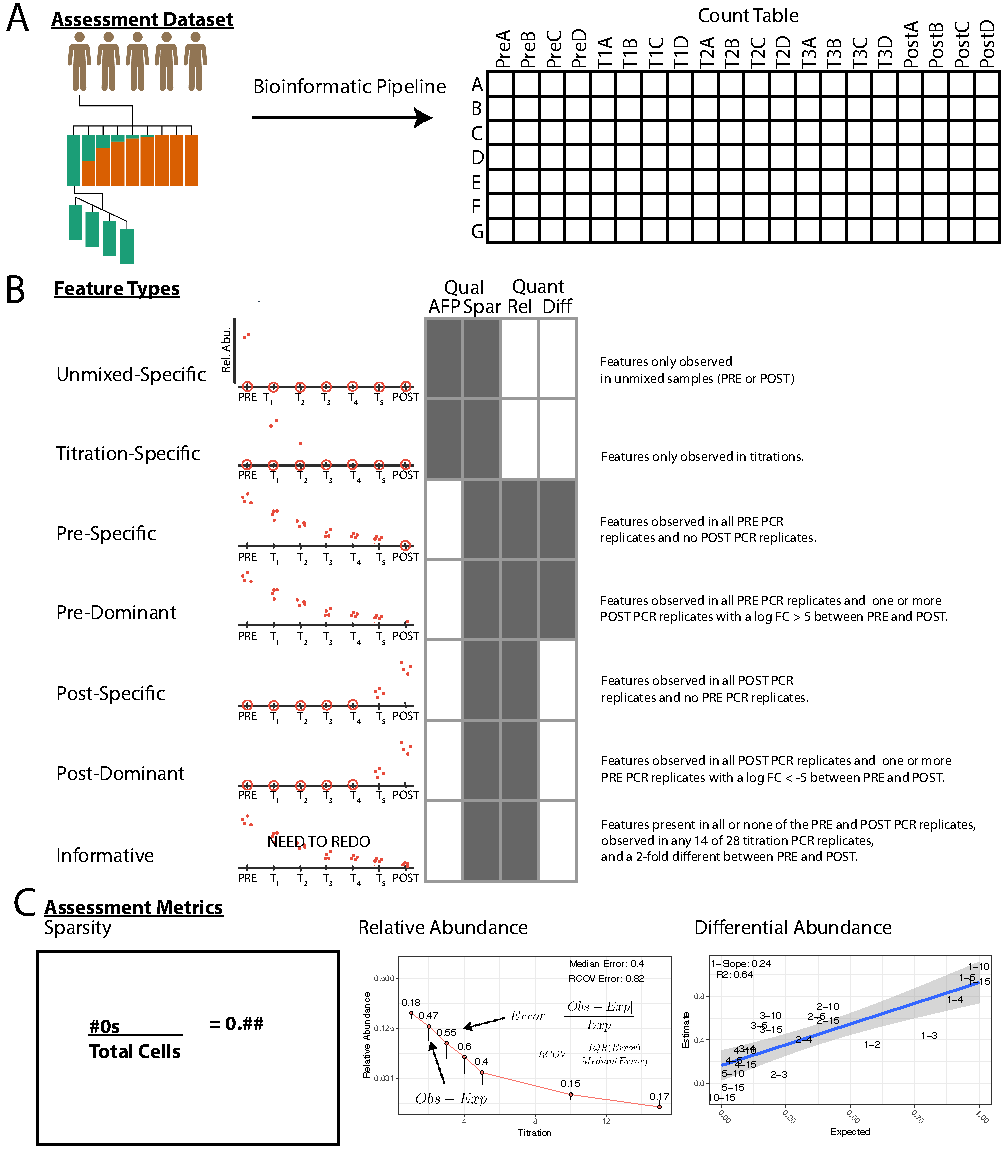
\includegraphics{AssessmentFramework.pdf}
\caption{\label{fig:assessmentFramework}Assessment Framework. A) Count tables evaluated by the assessment framework are generated from the assessment dataset using marker-gene survey bioinformatic pipelines. Count table rows are features identified by the bioinformatic pipeline and column are samples, four PCR replicates (labeled A-D) were sampled for PRE and POST and titrations, to simplify the diagram only three titrations are shown. B) Pictorial depiction of abundance values of the seven feature types observed and used in the assessment framework. C) Qualitative and quantitative assessment metrics used in the assessment framework. The artifactual feature proportion metric (AFP) is a qualitative assessment of feature presence/absence based on unmixed-specific or titration-specific artifactual features. Sparsity (SPAR) is a qualitative assessment of the proportion of observed features in each sample relative to the total observed features. Relative abundance metric (Rel) plot is a quantitative assessment of the relationship between the observed and expected relative abundance values. The difference is used to calculate the error rate ($|Obs-Exp|/Exp$) from which the bias metric ($median(error)$) and variance metric ($RCOV$) are calculated. The differential abundance (Diff) metric assesses the relationship between the expected log fold-change and estimated log fold-change is shown. Points represent the log fold-change between two titrations, point text indicates the titrations compared. A linear model is fit to the data. The model fit information is used for the differential abundance bias ($1-slope$) and variance metrics ($R^2$). Each feature type in (B) is labeled with the assessments shown in (C) in which they are employed.}
\end{figure}

Our framework assesses the qualitative and quantitative characteristics of the 16S rRNA measurement process (Fig. \ref{fig:assessmentFramework}).
The framework evaluates count tables generated by bioinformatic pipelines from a dataset developed specifically for use in this framework.
The qualitative assessment provides insight into how much confidence a user can have in feature  presence/absence.
The quantitative assessment evaluates the bias and variance of relative and differential abundance estimates.

\begin{figure}
\centering
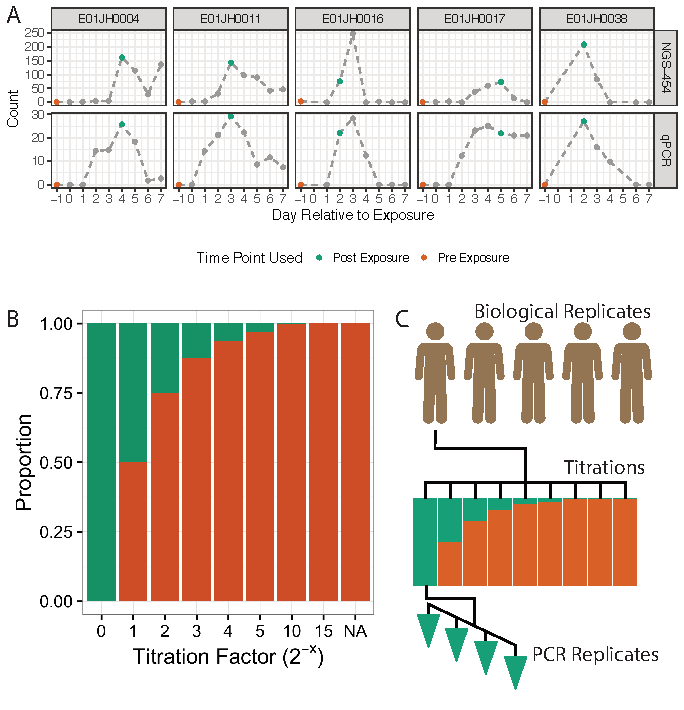
\includegraphics{experimentalDesign.pdf}
\caption{\label{fig:countExperimentalDesign}Sample selection and
experimental design for the two-sample titration 16S rRNA
marker-gene-survey assessment dataset. A) Pre- and post-exposure (PRE
and POST) samples from five vaccine trial participants were selected
based on \textit{Escherichia coli} abundance measured using qPCR and 454
16S rRNA sequencing (454-NGS), data from Pop et al. \cite{pop2016individual}.
Counts represent normalized relative abundance values for 454-NGS and
copies of the heat-labile toxin gene per \(\mu L\), a marker gene for
ETEC, for qPCR. PRE and POST samples are indicated with orange and green
data points, respectively. Grey points are other samples from the
vaccine trial time series. B) Proportion of DNA from PRE and POST
samples in titration series samples. PRE samples were titrated into POST
samples following a \(log_2\) dilution series. The NA titration factor
represents the unmixed PRE sample. C) PRE and POST samples from the five
vaccine trial participants, subjects, were used to generate independent
two-sample titration series. The result was a total of 45 samples, 7
titrations + 2 unmixed samples times 5 subjects. Four replicate PCRs
were performed for each of the 45 samples resulting in 190 PCRs.}
\end{figure}

\subsubsection*{Assessment Dataset - Mixture Design}

Using mixtures of environmental samples we generated a dataset with expected values for use in our assessment framework. 
For mixture datasets, expected values can be obtained using information from unmixed samples and the mixture design.
Our mixture dataset uses a two-sample titration mixture design, where DNA collected from five vaccine trial participants before and
after exposure to pathogenic \emph{Escherichia coli} was mixed following a \(log_2\) dilution series (Fig. \ref{fig:countExperimentalDesign}).
Each sample was sequenced in quadruplicate.
For our two-sample titration mixture design, expected feature
relative abundance is calculated using equation \eqref{eq:mixEq},
where \(\theta_i\), is the proportion of POST DNA in titration \(i\),
\(q_{ij}\) is the relative abundance of feature \(j\) in titration
\(i\), and the relative abundance of feature \(j\) in the unmixed PRE
and POST samples is \(q_{pre,j}\) and \(q_{post,j}\).
Throughout the rest of the manuscript, samples collected prior to and after \emph{E. coli} exposure are referred to as PRE and POST respectively.

\begin{equation}
  q_{ij} = \theta_i q_{post,j} + (1 - \theta_i) q_{pre,j}
  \label{eq:mixEq}
\end{equation}

\subsubsection*{Qualitative Assessment}
The qualitative assessment shows how well pipelines differentiate true biological sequences from measurement process artifacts.
Inadequate processing of artifacts results in false positive and false negative features where false positives are features in a count table that are not present in the sequenced sample and false negative features are biological sequences in a sample not represented in the count table.
Our qualitative assessment methods characterize the artifactual feature proportion (the frequency of artifactual features in a count table) by estimating the proportion of \emph{titration-} and \emph{unmixed-specific} features (Fig. \ref{fig:assessmentFramework}B) that cannot be explained by sampling alone.
We combine the artifactual feature proportion assessment results with sparsity estimates to hypothesize whether the artifactual features are primarily false positives or negatives.
Sparsity is defined as the fraction of 0 valued cells in the count table (Fig. \ref{fig:assessmentFramework}C).

\subsubsection*{Quantitative Assessment}
To evaluate count table abundance values, our quantitative assessment uses error, bias, and variance metrics (Fig. \ref{fig:assessmentFramework}C).
Error metrics measure agreement between observed and expected abundance values.
The bias and variance metrics summarise feature-level performance. 
Bias metrics summarise the overall agreement with expected values and the variance metric characterizes the distribution of the agreement.
Overall, pipeline performance is evaluated by comparing count table metric distributions.
Additionally, feature-level metrics are indicators of feature-specific biases.

\subsection*{Assessment Dataset Characterization and Validation}
To assure the mixture dataset is suitable for use in our assessment framework, we first validated the titration series and raw sequence data.
The mixture dataset had sufficient sample coverage, reads per sample, and read quality for use in our assessment framework. 
The number of reads per sample and distribution of base quality scores by position was consistent across subjects (Fig. S5).
There were \(8.9548\times 10^{4}\) (152,267 - 3,195) sequences per sample, median and
range. Average base quality score was greater than 30 over the length of the amplicon when considering both forward and reverse reads (Fig. S5B).

Additionally, we characterized subject specific differences to inform the interpretation of our assessment results.
No subject specific differences in base quality score were observed (Fig. S5). However, average read depth was greater for E01JH004 compared to the other individuals (Fig. S5).
Community composition differences between PRE and POST samples and individuals was characterized using alpha and beta diversity (Fig. S6). 
Overall alpha diversity was higher for POST except for E01JH0011, 
though differences in diversity between PRE and POST varied by individual. 
Based on the beta diversity the community composition within individuals differed between the PRE and POST samples. Note that assessment metrics defined above and results reported below are based on within subject comparisons.

To validate the two-sample titration assessment dataset,
we evaluated two assumptions about the titrations:
(1) The samples were mixed volumetrically in a
\(log_2\) dilution series according to the mixture design.
(2) The unmixed PRE and POST samples
have the same proportion of prokaryotic DNA.
To validate the sample volumetric mixing exogenous DNA (ERCC plasmids) were spiked into the
unmixed samples before mixing and quantified
using qPCR (Fig. S1B). The stool samples used to generate the mixtures have both eukaryotic (primarily human) DNA and
prokaryotic DNA. If the proportion of prokaryotic DNA differs between
the unmixed samples, then the amount of DNA from the unmixed samples in
a titration targeted by 16S rRNA gene sequencing is not consistent with
the mixture design. We quantified the proportion of prokaryotic DNA in the unmixed samples using a qPCR assay targeting the 16S rRNA gene (Fig. S1C).

Our assessment dataset validation results indicated that the samples were volumetrically mixed according to the mixture design (Table S1) but prokaryotic DNA proportion varied across the titration series (Fig. S2). 
To account for deviations from the mixture design due to differences in the proportion of prokaryotic DNA in the unmixed samples, we estimated the proportion of POST in each titration using the 16S rRNA sequencing data (Fig. S3) and 
the estimated POST proportions were used in our assessment metric calculations. 
See Supplemental Material for the assessment dataset validation methods and results.


\subsection*{Count Table Assessment Demonstration}
Next, we demonstrate the utility of our assessment framework on count tables generated using three different bioinformatic pipelines; DADA2, Mothur and QIIME.
First, we provide high level summary statistics for initial insight into how the count tables differ.
Next, we compare the assessment framework results for the three count tables.

\paragraph{Count Table Characteristics}
\begin{table}
\caption{\label{tab:pipeQA}Summary statistics for the different bioinformatic pipelines.
DADA2 is a denoising sequence inference pipeline, QIIME is an open-reference clustering
pipeline, and Mothur  is a de-novo clustering pipeline. No template controls were excluded
from summary statistics. Sparsity is the proportion of 0's in the count table. Features
is the total number of OTUs (QIIME and Mothur ) or SVs (DADA2) in the count. Sample
coverage is the median and range (minimum-maximum) per sample total abundance.
Drop-out rate is the proportion of reads removed while processing the sequencing data for each bioinformatic pipeline.}
\centering
\begin{tabular}[t]{lrrll}
\toprule
Pipelines & Features & Sparsity & Total Abundance & Drop-out Rate\\
\midrule
DADA2 & 3144 & 0.93 & 68649 (1661-112058) & 0.24 (0.18-0.59)\\
Mothur & 38358 & 0.98 & 53775 (1265-87806) & 0.4 (0.35-0.62)\\
QIIME & 11385 & 0.94 & 25254 (517-46897) & 0.7 (0.62-0.97)\\
\bottomrule
\end{tabular}
\end{table}

The count tables generated using the three bioinformatic pipelines vary in
pre-processing and feature inference methods. 
These differences are reflected in the count table number of features, total abundance,
and drop-out rate (Table \ref{tab:pipeQA}, Fig. S7B). The
pipelines evaluated employ different approaches for handling low quality
reads resulting in large differences in the drop-out rate, fraction
of raw sequences not included in the count table (Table
\ref{tab:pipeQA}). QIIME pipeline has the highest drop-out rate and
number of features per sample but fewer total features than Mothur. The
targeted amplicon region has a relatively small overlap region, 136 bp
for 300 bp paired-end reads, compared to other commonly used amplicons
\cite{kozich2013development, Walters2016-lf}. The high drop-out rate is
due to low basecall accuracy at the ends of the reads especially the
reverse reads resulting in a high proportion of unsuccessfully merged
reads pairs (Fig. S5B). Further increasing the
filter rate, QIIME excludes singletons (features only observed once in
the dataset).


Feature taxonomic composition also varied by pipeline (Fig. S8). 
The three pipelines generated unique feature sets in terms of sequence
length and amplicon position (see pipeline description). Therefore, we
used feature taxonomic assignments for cross-pipeline community composition comparison.
Phylum and order relative abundance is similar
across pipelines (Fig. S8A \& B). The observed
differences are attributed to different taxonomic classification methods
and databases used by the pipelines. Regardless
of the relative abundance threshold, most genera were
unique to individual pipelines (Fig. S8C \& D). Sets (shared taxa between pipelines) with QIIME had the fewest genera,
excluding the DADA2-QIIME set. QIIME was the only pipeline to use
open-reference clustering and the Greengenes database. Mothur and DADA2
both used the SILVA dataset. The Mothur and DADA2 pipeline use different
implementations of the RDP naïve Bayesian classifier, which may be
partially responsible for the Mothur, unclustered, and DADA2
differences.

\subsubsection*{Qualitative Assessment}

\begin{figure}
\centering
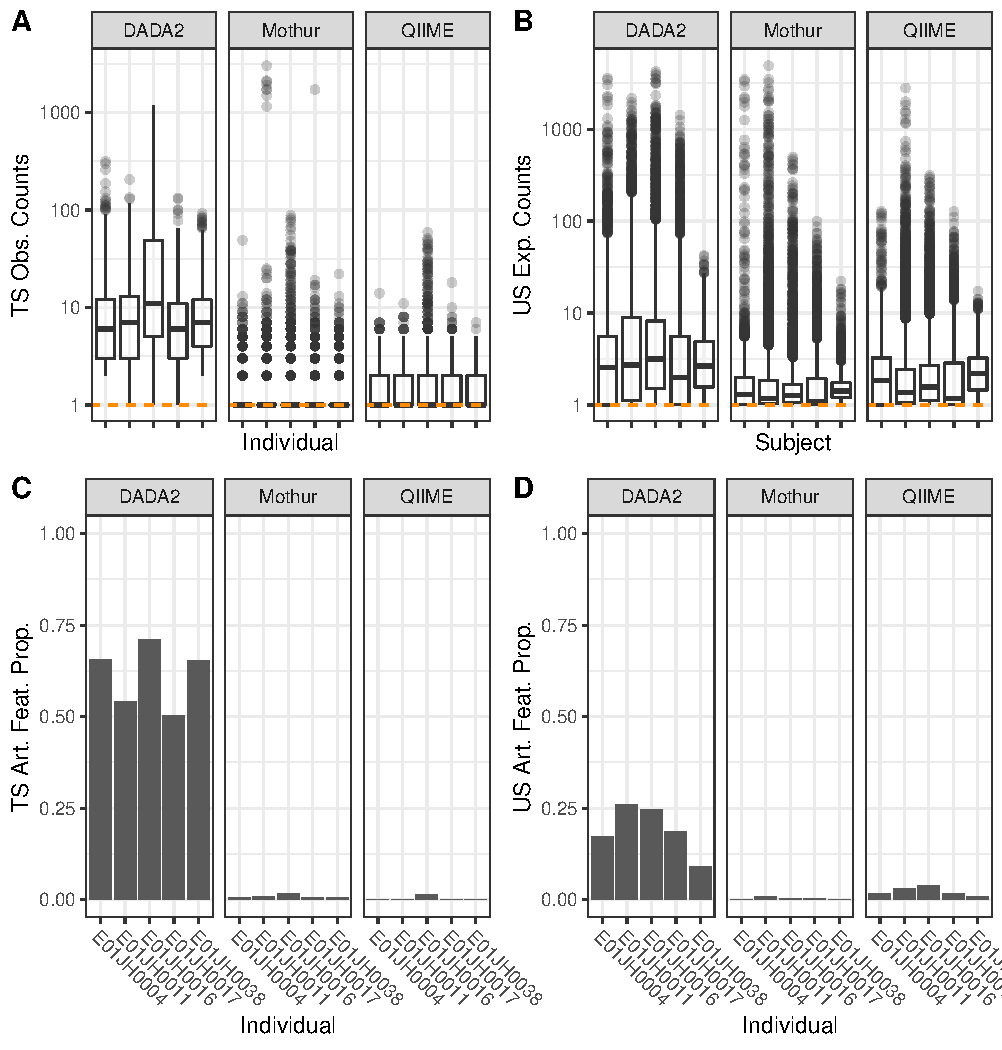
\includegraphics{qualPlot-1.pdf}
\caption{\label{fig:qualPlot}Distribution of (A) observed count values for
\emph{titration-specific} (TS) features and (B) expected count values for
\emph{unmixed-specific} (US) features by pipeline and individual. The orange
horizontal dashed line indicates a count value of 1. (C) Artifactual feature proportion (Art. Feat. Prop.) for
\emph{titration-specific} and (D) \emph{unmixed-specific} features with an
adjusted p-value \textless{} 0.05 for the Bayesian hypothesis test and
binomial test respectively. We failed to accept the null hypothesis when
the p-value \textless{} 0.05, indicating that the discrepancy between
the feature only being observed in the titrations or unmixed samples
cannot be explained by sampling alone.}
\end{figure}

To evaluate feature presence-absence, the framework's qualitative assessment measures
artifactual feature proportion and count table sparsity.
Low abundance features
present only in unmixed samples or titration samples are expected due to random
sampling. \emph{Unmixed-} and \emph{titration-specific} features were observed for all pipelines
(\emph{titration-specific}: Fig. \ref{fig:qualPlot}A, \emph{unmixed-specific}: Fig.
\ref{fig:qualPlot}B). Overall, the DADA2 count table had the largest
number of artifactual features (Table S3). 
A summary of the \emph{titration-specific} artifactual features is provided in the supplementary material.

We next assessed the proportion of these artifactual features that could be explained by sampling effects alone. For our two-sample titration dataset, there were
\emph{unmixed-specific} features with expected counts not which could not be explained by sampling
alone for all individuals and bioinformatic pipelines (Fig.
\ref{fig:qualPlot}C). However, the proportion of \emph{unmixed-specific}
features that could not be explained by sampling alone varied by
bioinformatic pipeline. DADA2 had the highest proportion of
\emph{unmixed-specific} artifactual features whereas QIIME had
the lowest proportion which is consistent with the distribution
of \emph{titration-specific} feature observed counts (Fig. \ref{fig:qualPlot}D).


We expected this mixture dataset to be less sparse relative to other datasets due
to the redundant nature of the samples where the 35 titration samples are derived
directly from the 10 unmixed samples, along with four PCR replicates for
each sample. We observed overall sparsity of 0.93 and 0.94 for DADA2 and QIIME respectively, and a higher value of 0.98 for Mothur \ref{tab:pipeQA}). 

To account for differences in microbial community composition across the five individuals we also measured sparsity at the individual level (Table S2).
Sparsity at the individual-level is lower than overall sparsity for all three pipelines. In this case, average sparsity across individuals for 0.70 and 0.76 for DADA2 and Mothur, while QIIME had a lower average sparsity across individuals of 0.56. Differences in alpha and beta diversity for the five individual unmixed samples are consistent with individual level sparsity and therefore reflects differences in individual microbial community composition.


Based on the artifactual feature proportions and count table sparsity, 
DADA2 artifactual features are likely due to false negative features, whereas the Mothur and QIIME high sparsity values were attributed to false positive features. 
Based on the observed sparsity levels it is unlikely that any of the pipelines successfully filtered out a
majority of the sequencing artifacts. Both unmixed- and titration-specific
features that can and cannot be explained by sampling alone contribute
to sparsity and the differences in the artifactual feature proportion
and sparsity provide insight into how the pipelines treat sequencing artifacts.


\subsubsection*{Quantitative Assessment}

\begin{figure}
\centering
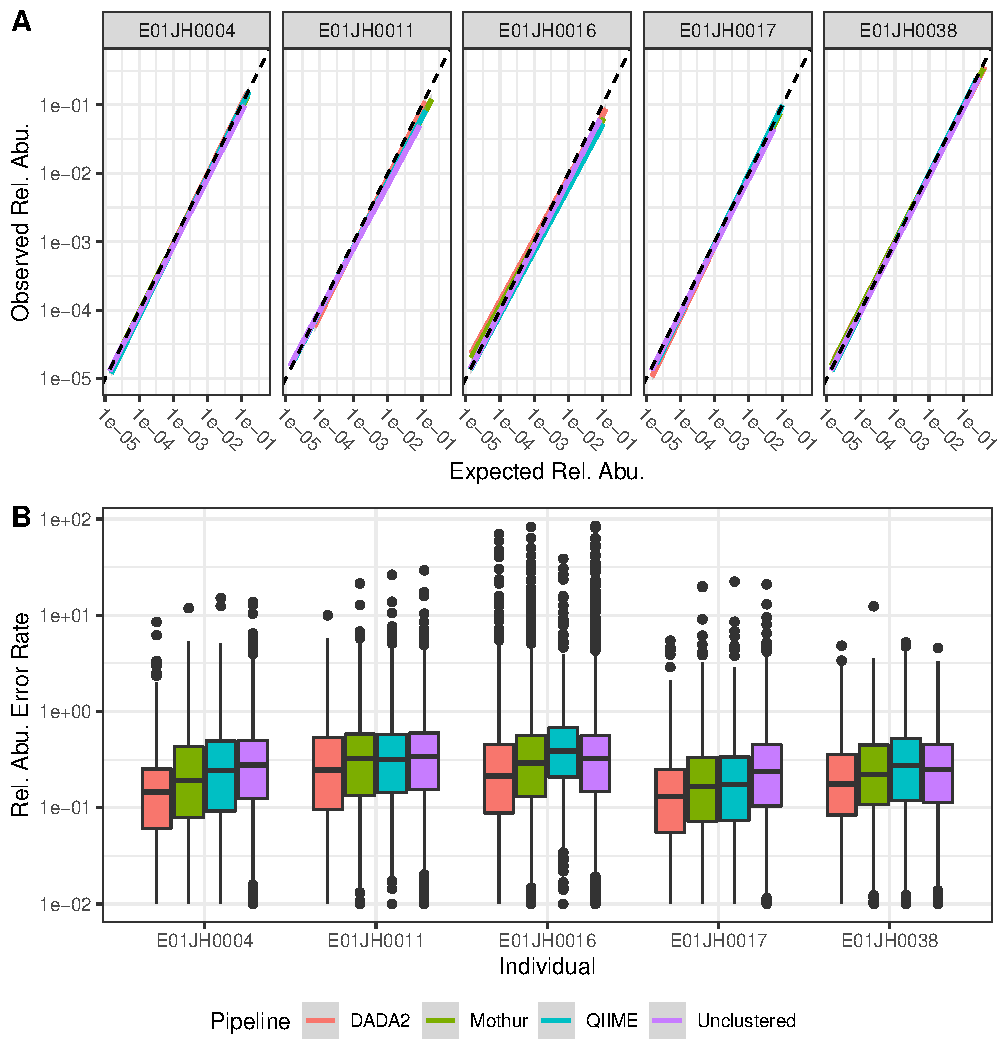
\includegraphics{relAbuError-1.pdf}
\caption{\label{fig:relAbuError}Relative abundance assessment.
(A) A linear model of the relationship between the expected and observed relative
abundance. The dashed grey line indicates expected 1-to-1 relationship.
The plot is split by individual and bioinformatic pipeline indicated by
line color. A negative binomial model was used to
calculate an average relative abundance estimate across PCR
replicates. To highlight quantitative performance for higher abundance features,
points with observed and expected relative abundance values less
than 1/median(total abundance) were excluded from the plot.
(B) Relative abundance error rate (\(|expected - observed|/expected\))
distribution by individual and pipeline.}
\end{figure}

\begin{figure}
\centering
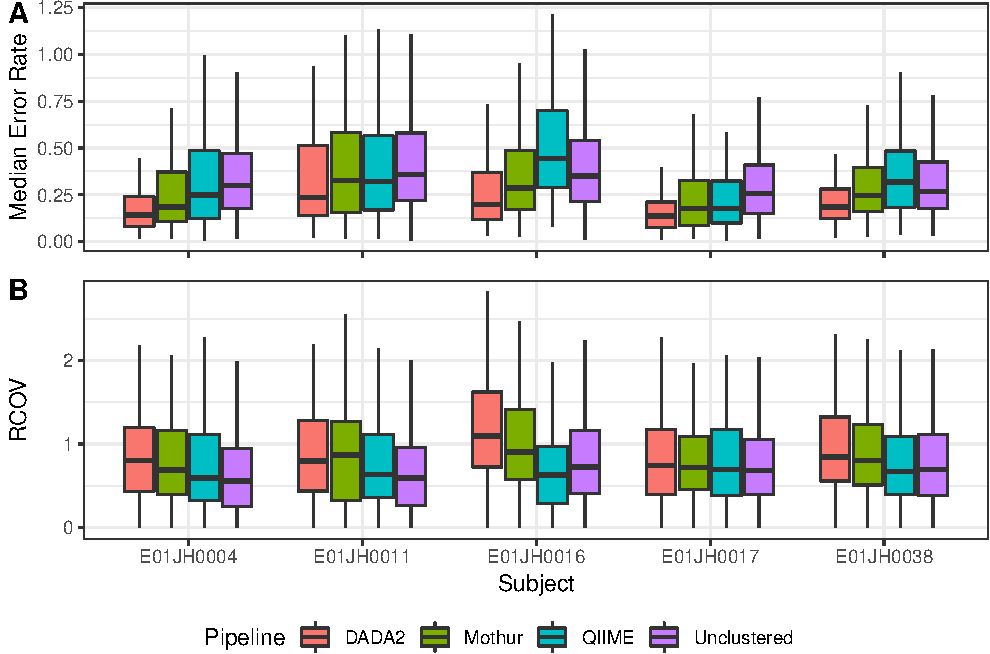
\includegraphics{relAbuErrorMetrics-1.pdf}
\caption{\label{fig:relAbuErrorMetrics}Comparison of pipeline relative
abundance assessment feature-level error metrics. Distribution of
feature-level relative abundance (A) bias metric - median error rate and
(B) variance - robust coefficient of variation (\(RCOV=IQR/|median error rate|\)) by individual and pipeline.
For both the bias and variance metrics lower values are better.
Boxplot outliers, \(1.5\times IQR\) from the median were excluded from the figure to prevent extreme metric values
from obscuring metric value visual comparisons.}
\end{figure}


\paragraph{Relative Abundance Assessment}
To assess count table feature relative abundance values, we evaluated the consistency of
the observed and expected relative abundance estimates for a feature and
titration as well as feature-level bias and variance.
Only features observed in all PRE and POST PCR replicates
and PRE and POST specific features were included in the analysis (Table S3). Overall, agreement between inferred
and observed relative abundance was high for all individuals and
bioinformatic pipelines (Fig. \ref{fig:relAbuError}A). The error rate
distribution was similarly consistent across pipelines, including long
tails (Fig. \ref{fig:relAbuError}B).

To assess quantitative accuracy across pipelines, we compared the feature-level relative
abundance error rate bias and variance
using mixed effects models. To control for subject specific differences, 
subject was included in the model as a random effect.
Large bias and variance metric values were
observed for all pipelines (Table S3).
Feature-level relative abundance error rate bias (median error rate, Fig.
\ref{fig:relAbuErrorMetrics}A) was significantly different between
pipeline, but no statistically significant differences were observed
for the variance metric, (\(RCOV=(IQR)/|median|\), Fig.
\ref{fig:relAbuErrorMetrics}B) across pipeline. The Mothur, DADA2,
and QIIME feature-level biases were all significantly different from
each other (\(p < 1\times 10^{-8}\)). DADA2 had the lowest mean
feature-level bias (0.2), followed by Mothur (0.28), with QIIME having the highest bias
(0.33) (\ref{fig:relAbuErrorMetrics}B). Large variance metric values
were observed for all individuals and pipelines (Table S3). The feature-level variance was not
significantly different between pipelines: Mothur = 0.83, QIIME = 0.71
and DADA2 = 1 (Fig. \ref{fig:relAbuErrorMetrics}B).


\begin{figure}
\centering
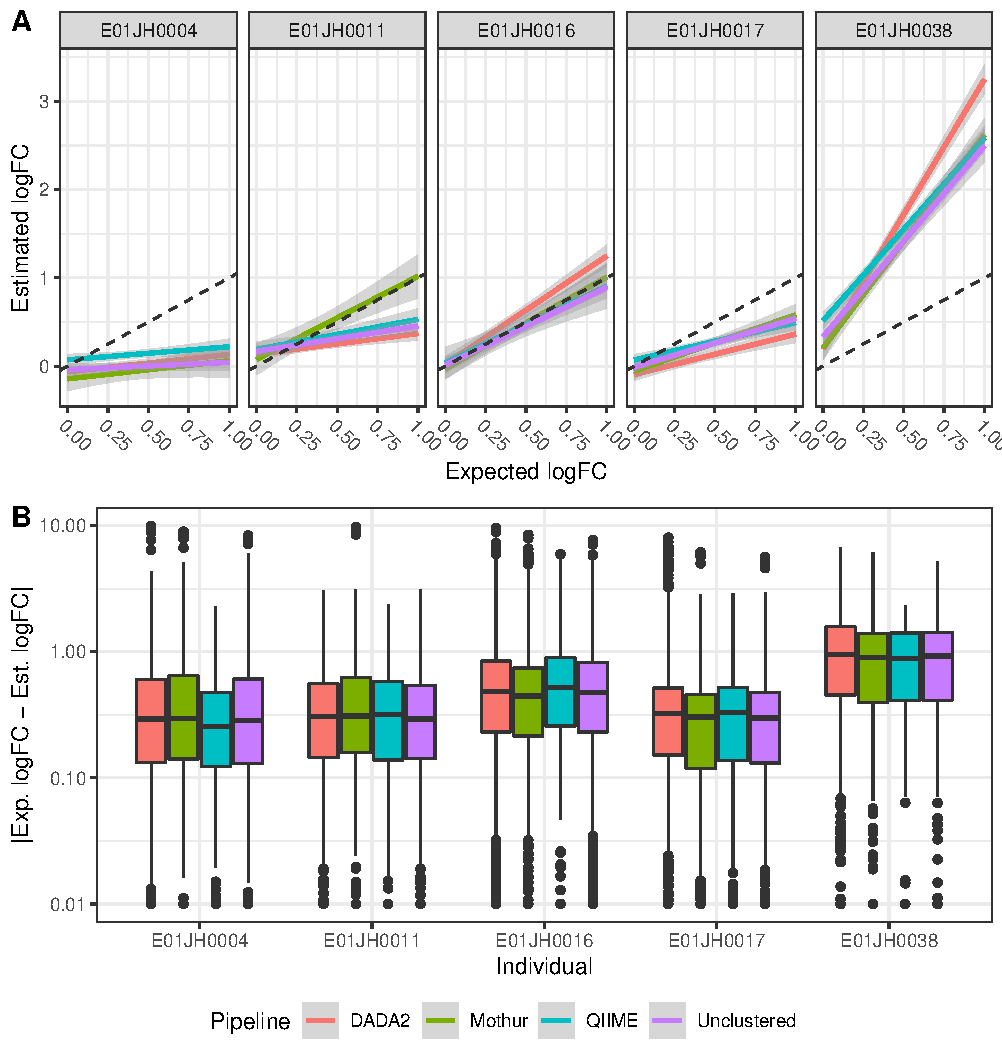
\includegraphics{logFCerror-1.pdf}
\caption{\label{fig:logFCerror} Differential abundance quantitative assessment. (A) Linear model of the relationship between
estimated and expected log fold-change relative abundance between titrations for PRE-specific and
PRE-dominant features by pipeline and individual, line color indicates
pipelines. Dashed grey line indicates expected 1-to-1 relationship
between the estimated and expected log fold-change. (B) Log fold-change
error (\textbar{}exp-est\textbar{}) distribution by pipeline and
individual.}
\end{figure}


\begin{figure}
\centering
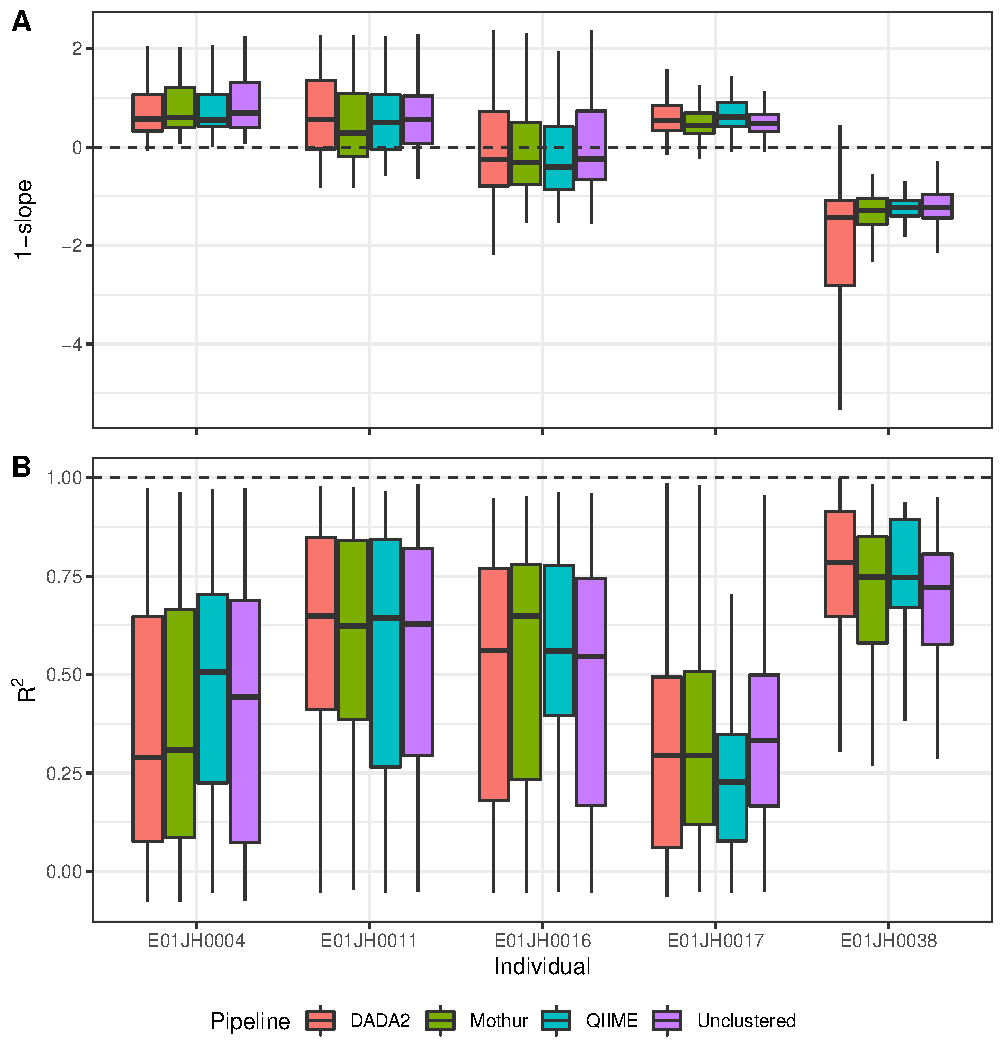
\includegraphics{logFcErrorMetrics-1.pdf}
\caption{\label{fig:logFcErrorMetrics}Feature-level differential abundance assessment.Log-fold change error
bias (A) and variance (B) metric distribution by subject and pipeline.
The bias (\(1 - slope\)) and variance (\(R^2\)) metrics are derived from
the linear model fit to the estimated and expected log fold-change
values for individual features. Boxplot outliers, \(1.5\times IQR\) from
the median were excluded from the figure to prevent extreme metric
values from obscuring metric value visual comparisons.}
\end{figure}

\paragraph{Differential Abundance Assessment}
The agreement between log-fold change estimates and expected values were
individual specific and consistent across pipelines (Fig.
\ref{fig:logFCerror}A). The individual specific effect was attributed to
the fact that unlike relative abundance assessment, the inferred
\(\theta\) values were not used to calculate expected values. Inferred
\(\theta\) values were not used to calculate the expected values because
all of the titrations and the \(\theta\) estimates for the higher
titrations were not monotonically decreasing.
Using the inferred \(\theta\) resulted in unrealistic expected log fold-change values, e.g.,
negative log-fold changes for PRE specific features. The log-fold change
estimates and expected values were consistent across pipelines with one
notable exception: for subject E01JH0011, the Mothur log fold-change estimates
were more consistent with expected values than the other pipelines.
However, as \(\theta\) was not corrected for differences in the
proportion of prokaryotic DNA between the unmixed PRE and POST samples,
it cannot be said whether Mothur's performance was better than the other
pipelines.


The log fold-change error distribution was consistent across pipelines
(Fig. \ref{fig:logFCerror}B). There was a long tail of high error
features in the error distribution for all pipelines and individuals.
The log fold-change estimates responsible for the long tail could not be
attributed to specific titration comparisons. Additionally, we compared
error distributions for log-fold change estimates using
different normalization methods. Error rate distributions, including the
long tails, were consistent across normalization methods. Seeing
as the long tail was observed for the unclustered data as well, the
log-fold change estimates contributing to the long tail are likely due
to a bias associated with the molecular portion of the
measurement process and not the computational portion. Exploratory
analysis of the relationship between the log fold-change estimates and
expected values for individual features indicated that the long tails
were attributed to feature specific performance.

Feature-level log fold-change bias and variance metrics were used to
compare pipeline performance (Fig. \ref{fig:logFCerror}). Similar to
relative abundance, feature-level bias and variance metrics are defined
as the \(1 - slope\) and \(R^2\) for linear models of the estimated and
expected log fold-change for individual features and all titration
comparisons. For the bias metric, \(1 - slope\), the desired value is 0
(i.e., log fold-change estimate = log fold-change expected), with
negative values indicating the log-fold change was consistently
underestimated and positive values consistently overestimated. The
linear model \(R^2\) value was used to characterize the feature-level
log fold-change variance as it indicates consistency between log
fold-change estimates and expected values across titration comparisons.
To compare bias and variance metrics across pipelines, mixed-effects
models were used. The log fold-change bias and variance metrics were not
significantly different between pipelines (Bias: F = 0, 2.51, p = 0.99,
0.08, \ref{fig:logFCerror}B, Variance: F = 47.39, 0.23, p = 0, 0.8, Fig.
\ref{fig:logFCerror}C).


\section*{Discussion}
Mixtures of environmental samples have been used to assess
RNAseq and microarray gene expression measurements \cite{parsons2015using, pine2011adaptable, thompson2005use}.
However, this is the first time mixtures have been used to assess microbiome measurement
methods. We developed a novel assessment framework utilizing a mixture dataset
for evaluating marker-gene-survey computational methods (Fig. \ref{fig:assessmentFramework}).

Using mixtures of environmental samples, expected values for use in assessment
can be obtained using information from unmixed samples and how the samples were mixed.
Our assessment dataset follows a two-sample titration mixture design, where DNA collected from five vaccine trial participants before and
after exposure to pathogenic \emph{Escherichia coli}  was mixed following a \(log_2\) dilution
series (Fig. \ref{fig:countExperimentalDesign}).
Count table qualitative characteristics were assessed using relative abundance information for
features observed only in titrations (titration-specific) and unmixed samples (unmixed-specific) (Fig. \ref{fig:assessmentFramework}B).
Statistical tests were used to determine if the absence of unmixed-specific features from titrations or absence of titration-specific features from unmixed samples could be explained by random sampling.
Count tables were quantitatively assessed by comparing observed feature relative abundance and feature differential abundance estimates to expected values.
Quantitative performance was characterized using error rate, along with feature-level bias variance metrics we developed (Fig. \ref{fig:assessmentFramework}C).


\subsubsection*{Count Table Assessment Demonstration}
We demonstrated our assessment framework on count tables generated by three commonly used bioinformatic pipelines, QIIME, Mothur, and DADA2.
The objective of any pipeline is to differentiate true biological sequences from measurement process artifacts along with accurate abundance estimates.
Our qualitative assessment results, when combined with sparsity information provides a
new method for evaluating how well bioinformatic pipelines account for sequencing artifacts without loss of true biological sequences.
Additionally, our quantitative assessment results identified previously unknown feature specific biases in abundance estimates.

The qualitative assessment evaluates if titration- and unmixed-specific features can be explained by random sampling alone (Fig. \ref{fig:assessmentFramework}B).
Titration- and unmixed-specific features not explained by sampling are artifacts of the measurement process.
These artifacts can be viewed as false-positives, not representative of actual sequences in a sample,
or false-negatives, actual sequences in a sample not represented by count table features. 
Artifacts can be PCR errors such as chimeras, reads with high sequencing error rates, or cross sample contamination \cite{edgar2011uchime, Edgar2018-ss, damore2016}. 
Count table sparsity information (the proportion of zero-valued cells) provides
additional insight into the qualitative assessment results.

A high false negative rate provides an explanation for DADA2's high proportion
of artifact titration- and unmixed-specific features and count table having
comparable sparsity to the other pipelines despite having significantly fewer
features (Fig. S5 and Table \ref{tab:pipeQA}).
The DADA2 feature inference algorithm may be aggressively grouping
lower abundance true sequences with higher abundance sequences.
As a result, the low abundance sequences are not present in samples
leading to increased sparsity and high abundance unmixed- and titration-specific features.
This aggressive grouping of sequences is a design choice made by the algorithm developers.
The DADA2 documentation states that the default setting for \texttt{OMEGA\_A}
is conservative to prevent false positives at the cost of increasing false negatives \cite{callahan2016dada2}.
Using the qualitative assessment methods described here, a user can
adjust the \texttt{OMEGA\_A} parameter to obtain a false-negative rate appropriate for their study. 


While the relative abundance bias metric was significantly different
between pipelines, overall, pipeline choice had minimal impact on the
quantitative assessment results when accounting for subject-specific deviations
in the proportion of prokaryotic DNA from PRE and POST samples in a
titration from the mixture design. Outlier features (those with extreme bias
and variance metrics) were observed for all pipelines and both abundance assessments.

Outlier features could not be attributed to bioinformatic pipelines
and are likely due to biases in the molecular biology part of the measurement process.
Outlier features are unlikely pipeline artifacts as they were observed in count tables generated
using the unclustered pipeline as well as standard bioinformatic
pipelines. Additionally, we were unable to attribute outlier features to relative
abundance values, log fold-change between unmixed samples, and sequence
GC content. Furthermore, features with extreme metric values were not limited to any
specific taxonomic group or phylogenetic clade. PCR amplification
bias (a well-known source of bias in the molecular biology part of the
measurement process) is one possible explanation for the outlier features \cite{Sze565598}.
Mismatches in the primer binding regions impact PCR efficiency
and are a potential cause for poor feature-specific
performance \cite{wright2014exploiting}. Additional research is
needed before outlier features can be attributed to mismatches in the primer binding regions.

Based on our assessment results, we suggest using DADA2 for
feature-level abundance analysis, e.g.~differential abundance testing.
While DADA2 performed poorly in our qualitative assessment,
the pipeline performed better in the quantitative assessment compared to the other pipelines.
Additionally, the DADA2 poor qualitative assessment results due to
false-negative features are unlikely to negatively impact feature-level abundance analysis.
When determining which pipeline to use for a study, users should consider
whether minimizing false positives (DADA2) or false negatives (Mothur)
is more appropriate for their study objectives.
Based on our findings we find that users of DADA2 can be more
confident that an observed feature represents a member of the
microbial community and not a measurement artifact, but careful examination of sequences assigned to features of interest should still be performed.

\subsubsection*{Using Mixtures to Assess 16S rRNA Sequencing - Lessons Learned}

There are limitations using our assessment dataset, these include:
(1) Lack of agreement between the proportion of prokaryotic DNA from the
unmixed samples in the titrations and the mixture design.
(2) The mixture design resulted in a limited number of features and range of expected log-fold changes.
These limitations are described below along with
recommendations for addressing them in future studies.

Differences in the proportion of prokaryotic DNA in the samples used to
generate the two-sample titrations series resulted in differences
between the true mixture proportions and mixture design. We attempted to
account for differences in mixture proportion from mixture design by
using sequence data to estimate mixture proportions similar to how mRNA
proportions in RNA samples were used in a previous mixture study
\cite{parsons2015using}. We used an assay targeting the 16S rRNA gene
to detect changes in the concentration of prokaryotic DNA across
titrations, but were unable to quantify the proportion of prokaryotic
DNA in the unmixed samples using qPCR data. Using the 16S rRNA sequencing
data, we inferred the proportion of prokaryotic DNA from the POST sample
in each titration. However, the uncertainty and accuracy of the
inference method are not known, resulting in an unaccounted for source of error.

A better method for quantifying sample prokaryotic DNA proportion or
using samples with consistent proportions would increase confidence in
the expected value and, in-turn, error metric accuracy. Limitations in the
prokaryotic DNA qPCR assay's concentration precision limits the
assay's suitability for use in mixture studies. Digital PCR provides a
more precise alternative to qPCR and is, therefore, a more appropriate
method. Alternatively using samples where the majority of the DNA is
prokaryotic would minimize this issue. Mixtures of environmental samples
can also be used to assess shotgun metagenomic methods as well. As
shotgun metagenomics is not a targeted approach, differences in the
proportion of prokaryotic DNA in a sample would not impact the
assessment results in the same way as 16S rRNA marker-gene-surveys.

Using samples from a vaccine trial allowed for the use of a specific
marker with an expected response, \emph{E. coli}, during methods
development. However, the high level of similarity between the PRE and POST unmixed
samples resulted in a limited number of features that could be used in
the quantitative assessment results. Using more diverse samples to
generate mixtures would address this issue.
Alternatively, instead of mixing PRE and POST samples from the same individual,
mixing PRE and POST samples from different individuals would
have resulted in additional features for use in our quantitative assessment.
While unmixed sample similarity impacts the number of features
that can be used in the quantitative assessment, the qualitative
assessment is not impacted by unmixed sample similarity.
Finally, a symmetric mixture design, for example one with unmixed
PRE and POST ratios of 1:4, 1:2, 1:1, 2:1, and 4:1, would provide a larger
dynamic range of abundance values for assessing both PRE and POST specific features.


\section*{Conclusions}
Our assessment framework can be used to evaluate and characterize 16S rRNA marker-gene survey analysis methods, in particular count tables produced by any 16S rRNA bioinformatic pipeline.
We demonstrated our assessment framework with three commonly used bioinformatic pipelines.
Our qualitative assessment results indicated that the QIIME and Mothur pipelines produced count table with more false-positive features whereas the DADA2 count table had more false-negative features.
Overall the three pipelines performed well in our quantitative assessment. 
However, feature-level analysis identified poorly performing features and the sources of  
bias responsible for this poor feature-level quantitative performance are unknown. 
Therefore, feature-level results for any 16S rRNA marker-gene survey should be interpreted with care. 
Addressing both of these issues requires advances in both the molecular biology and
computational components of the measurement process.


\section*{Methods}

\subsection*{Assessment Framework}
To assess the qualitative and quantitative performance of marker-gene survey analysis methods we developed a framework utilizing our two-sample titration dataset(Fig. \ref{fig:assessmentFramework}).
Qualitative assessment evaluates feature presence-absence.
The quantitative assessment evaluates the relative and differential abundance estimates.

\subsubsection*{Assessment Dataset - Mixture Design}
To provide a dataset with real-world complexity and expected values for  qualitative and quantiative assessment we used mixtures of environmental samples.
Samples collected at multiple timepoints during a Enterotoxigenic
\emph{E. coli} (ETEC) vaccine trial \cite{harro2011refinement} were
used to generate a two-sample titration dataset (Fig.
\ref{fig:countExperimentalDesign}). Samples from five trial
participants were selected for our two-sample titration dataset. Trial
participants (subjects) and sampling timepoints were selected based on
\emph{E. coli} abundance data collected using qPCR and 16S rRNA
sequencing from Pop et al. \cite{pop2016individual}. Only individuals with no
\emph{E. coli} detected in samples collected from trial participants
prior to ETEC exposure (PRE) were used for our two-samples titrations.
Post ETEC exposure (POST) samples were identified as the timepoint after
exposure to ETEC with the highest \emph{E. coli} concentration for each
subject (Fig. \ref{fig:countExperimentalDesign}A). Due to limited sample
availability, for E01JH0016 the timepoint with the second highest
\emph{E. coli} concentration was used as the POST sample. Independent
titration series were generated for each subject. POST samples
were titrated into PRE samples with POST proportions of 1/2, 1/4, 1/8,
1/16, 1/32, 1/1,024, and 1/32,768 (Fig.
\ref{fig:countExperimentalDesign}B). Unmixed (PRE and POST) sample DNA
concentration was measured using NanoDrop ND-1000 (Thermo Fisher
Scientific Inc.~Waltham, MA USA). Unmixed samples were diluted to 12.5
\(ng/\mu L\) in tris-EDTA buffer before mixing. The resulting titration series
was composed of 45 samples, seven titrations and two unmixed samples for each
of the five subjects.

The 45 samples were processed using the Illumina 16S library protocol
(16S Metagenomic Sequencing Library Preparation, posted date 11/27/2013,
downloaded from \url{https://support.illumina.com}). This protocol
specifies an initial PCR of the 16S rRNA gene, followed by a sample indexing
PCR, sample concentration normalization, and sequencing.

A total of 192 16S rRNA PCR assays were sequenced across two 96-well plates including four PCR replicates
per sample and 12 no-template controls. The initial
PCR assay targeted the V3-V5 region of the 16S rRNA gene, Bakt\_341F and
Bakt\_806R \cite{klindworth2012evaluation}. The V3-V5 region is 464
base pairs (bp) long, with forward and reverse reads overlapping by 136
bp, using 2 X 300 bp paired-end sequencing \cite{yang2016sensitivity} (
\url{http://probebase.csb.univie.ac.at}). Primer sequences include
overhang adapter sequences for library preparation (forward primer 5'-
TCG TCG GCA GCG TCA GAT GTG TAT AAG AGA CAG CCT ACG GGN GGC WGC AG - 3'
and reverse primer 5'- GTC TCG TGG GCT CGG AGA TGT GTA TAA GAG ACA GGA
CTA CHV GGG TAT CTA ATC C - 3'). Kapa HiFi HotStart
ReadyMix reagents (KAPA Biosystems, Inc.~Wilmington, MA) was used to PCR the 16S rRNA gene. The PCR product amplicon size
was verified using agarose gel electrophoresis.
Concentration measurements were made after the initial 16S rRNA PCR, the
indexing PCR, and normalization steps. DNA concentration was measured
using the QuantIT Picogreen dsDNA Kit (Cat \# P7589, ThermoFisher
Scientific) and fluorescent measurements were made with a Synergy2
Multi-Detection MicroPlate Reader (BioTek Instruments, Inc, Winooski,
VT).


Initial PCR products were purified using 0.8X AMPure XP beads (Beckman
Coulter Genomics, Danvers, MA) following the manufacturer's protocol.
After purification, the 192 samples were indexed using the Illumina
Nextera XT index kits A and D (Illumina Inc., San Diego CA) and then
purified using 1.12X AMPure XP beads. Prior to pooling purified sample
concentration was normalized using SequalPrep Normalization Plate Kit
(Catalog n. A10510-01, Invitrogen Corp., Carlsbad, CA), according to the
manufacturer's protocol. Pooled library concentration was checked using
the Qubit dsDNA HS Assay Kit (Part\# Q32851, Lot\# 1735902,
ThermoFisher, Waltham, MA USA). Due to the low pooled amplicon library
DNA concentration, a modified protocol for low concentration libraries
was used. The library was run on an Illumina MiSeq, and base calls were
made using Illumina Real Time Analysis Software version 1.18.54.
The sequence data was deposited in the NCBI SRA archive under Bioproject
PRJNA480312. Individual SRA run accession numbers and metadata in Supplemental Table.
Sequencing data quality control metrics for the 384 fastq sequence files
(192 samples with forward and reverse reads) were computed using the
Bioconductor \texttt{Rqc} package \cite{Rqc, Bioconductor}.


Sequence data were processed using four bioinformatic pipelines: a
\emph{de-novo} clustering method - Mothur
\cite{schloss2009introducing}, an open-reference clustering method -
QIIME \cite{Caporaso2010}, and a sequence inference method - DADA2
\cite{callahan2016dada2}, and unclustered sequences as a control. The
code used to run the bioinformatic pipelines is available at
\url{https://github.com/nate-d-olson/mgtst_pipelines}.

The Mothur pipeline follows the developer's MiSeq SOP
\cite{schloss2009introducing, kozich2013development}. The pipeline was
run using Mothur version 1.37 (\url{http://www.mothur.org/}). We
sequenced a larger 16S rRNA region, with smaller overlap between the
forward and reverse reads, than the 16S rRNA region the SOP was
designed. Pipeline parameters modified to account for difference in
overlap are noted for individual steps below. The Makefile and scripts
used to run the Mothur pipeline are available
\url{https://github.com/nate-d-olson/mgtst_pipelines/blob/master/code/mothur}.
The Mothur pipeline includes an initial preprocessing step where the
forward and reverse reads are trimmed and filtered using base quality
scores and were merged into single contigs for each read pair. The
following parameters were used for the initial contig filtering, no
ambiguous bases, max contig length of 500 bp, and max homopolymer length
of 8 bases. For the initial read filtering and merging step, low-quality
reads were identified and filtered from the dataset based on the
presence of ambiguous bases, failure to align to the SILVA reference
database (V119, \url{https://www.arb-silva.de/}) \cite{quast2012silva},
and identification as chimeras. Prior to alignment, the SILVA reference
multiple sequence alignment was trimmed to the V3-V5 region, positions
6,388 and 25,316. Chimera filtering was performed using UChime (version
v4.2.40) without a reference database \cite{edgar2011uchime}. OTU
clustering was performed using the OptiClust algorithm with a clustering
threshold of 0.97 \cite{westcott2017opticlust}. The RDP classifier
implemented in Mothur was used for taxonomic classification against the
Mothur provided version of the RDP v9 training set
\cite{wang2007naive}.

The QIIME open-reference clustering pipeline for paired-end Illumina
data was performed according to the online tutorial (Illumina Overview
Tutorial (an IPython Notebook): open reference OTU picking and core
diversity analyses, \url{http://qiime.org/tutorials/}) using QIIME
version 1.9.1 \cite{Caporaso2010}. Briefly, the QIIME pipeline uses
fastq-join (version 1.3.1) to merge paired-end reads
\cite{aronesty2011ea} and the Usearch algorithm \cite{edgar2010search}
with Greengenes database version 13.8 with a 97\% similarity threshold
\cite{desantis2006greengenes} was used for open-reference clustering.

DADA2, an R native pipeline was also used to process the sequencing data
\cite{callahan2016dada2}. The pipeline includes a sequence inference
step and taxonomic classification using the DADA2 implementation of the
RDP naïve Bayesian classifier \cite{wang2007naive} and the SILVA
database V123 provided by the DADA2 developers
\cite[\url{https://benjjneb.github.io/dada2/training.html}]{quast2012silva}.

The unclustered pipeline was based on the Mothur \emph{de-novo}
clustering pipeline, where the paired-end reads were merged, filtered,
and then dereplicated. Reads were aligned to the reference Silva
alignment (V119, \url{https://www.arb-silva.de/}), and reads failing
alignment were excluded from the dataset. Taxonomic classification of
the unclustered sequences was performed using the same RDP classifier
implemented in Mothur used for the \emph{de-novo} pipeline. To limit the
size of the dataset the most abundant 40,000 OTUs (comparable to the
Mothur dataset), across all samples, were used as the unclustered
dataset.


\subsubsection*{Qualitative Assessment}
\paragraph*{Artifactual Feature Proportion}
Our qualitative assessment evaluated features only observed in unmixed samples (PRE or POST) or only in titrations.
The former we will refer to as unmixed-specific features and the latter we will refer to as titration-specific features (Fig. \ref{fig:assessmentFramework}B).
\emph{Unmixed-} and \emph{titration-specific} features can arise from errors in the PCR/sequencing, feature inference processes, or due to differences in sampling depth. 
To provide context for the artifactual feature proportion results count table sparsity was used (Fig. \ref{fig:assessmentFramework}C).
Sparsity is defined as the proportion of 0 valued cells in a matrix.

Hypothesis tests were used to determine if random sampling alone, here sequencing depth, could account for \emph{unmixed-} and \emph{titration-specific} features.
p-values were adjusted for multiple comparisons using the Benjamini \& Hochberg method \cite{benjamini1995controlling}.
For \emph{unmixed-specific} features, a binomial test was used to evaluate if true feature relative abundance is less than the expected relative abundance.
The binomial test was infeasible for \emph{titration-specific} features.
Because the count table abundance values for these features was 0 in the unmixed samples,
their estimated probability of occurrence $\pi_{min}$ is equal to 0,
and thus, the binomial test fails.
Therefore, we formulated a Bayesian hypothesis test for \emph{titration-specific} features detailed by equation \eqref{eq:bht}.
This Bayesian approach was used to  evaluate if the true feature proportion is less than the minimum detected proportion.
Note that when assuming equal priors, $P(\pi < \pi_{min}) = P(\pi > \pi_{min})$,
\eqref{eq:bht} reduces to \eqref{eq:bht2}.
We define $\pi$ as the true feature proportion, $\pi_{min}$ the minimum detected proportion,
$C$ the expected feature counts, and $C_{obs}$ the observed feature counts.
Count values for $C$ were simulated using a beta prior (with varying alpha and beta values) for $\pi > \pi_{min}$ and a uniform distribution for $\pi < \pi_{min}$.
Higher values of alpha and beta will skew the prior right and left respectively. Our Bayesian hypothesis tests (Eg. \eqref{eq:bht2}) results were largely unaffected by beta distribution parameterization (Fig. S4).
$\pi_{min}$ was calculated using the mixture equation \eqref{eq:mixEq} where $q_{pre,j}$ and $q_{post,j}$ are $min(\textbf{Q}_{pre})$ and $min(\textbf{Q}_{post})$ across all features for a subject and pipeline.
Our assumption is that $\pi$ is less than $\pi_{min}$ for features not observed in unmixed samples.
Artifacts not explained by sequencing alone are likely errors in the sequence measurement and inference processes, and thus, false positives or negatives.


\begin{equation}
  \begin{split}
    p & = P(\pi < \pi_{min} | C \geq C_{obs}) \\
      & = \frac{P(C \geq C_{obs}| \pi < \pi_{min})P(\pi < \pi_{min})}{P(C \geq C_{obs}| \pi < \pi_{exp})P(\pi < \pi_{min}) + P(C \geq C_{obs}| \pi \geq \pi_{min})P(\pi \geq \pi_{min})} \\
  \end{split}
  \label{eq:bht}
\end{equation}

\begin{equation}
    p = \frac{P(C \geq C_{obs}| \pi < \pi_{min})}{P(C \geq C_{obs})}
  \label{eq:bht2}
\end{equation}



\subsubsection*{Quantitative Assessment}
For quantitative assessment, we compared observed relative abundance and
log fold-changes to expected values derived from the titration
experimental design.
Feature average relative abundance across PCR
replicates was calculated using a negative binomial model, and used as
observed relative abundance values (\(obs\)) for the relative abundance
assessment. Average relative abundance values were used to reduce PCR
replicate outliers from biasing the assessment results. Equation
\eqref{eq:mixEq} and inferred \(\theta\) values were used to calculate the
expected relative abundance values (\(exp\)). Relative abundance error
rate is defined as \(|exp - obs|/exp\).
We developed bias and variance metrics to assess feature performance.
The feature-level bias and variance metrics were defined as the median
error rate and robust coefficient of variation (\(RCOV=IQR/median\))
respectively.

Log fold-change between samples in the titration series including PRE
and POST were compared to the expected log fold-change values to assess
differential abundance log fold-change estimates. Log fold-change
estimates were calculated using EdgeR
\cite{Robinson2010, McCarthy2012}. Expected log fold-change for feature
\(j\) between titrations \(l\) and \(m\) is calculated using equation
\eqref{eq:expLogFC}, where \(\theta\) is the proportion of POST bacterial
DNA in a titration, and \(q\) is feature relative abundance. For
features only present in PRE samples, the expected log fold-change is
independent of the observed counts for the unmixed samples and is
calculated using \eqref{eq:expPreLogFC}. Features only observed in POST
samples, \emph{POST-specific}, expected log fold-change values can be
calculated in a similar manner. However, \emph{POST-specific} features
were rarely observed in more than one titration and therefore were not
suitable for use in our assessment. Due to a limited number of
\emph{PRE-specific} features, both \emph{PRE-specific} and
\emph{PRE-dominant} features were used in the differential abundance
assessment. \emph{PRE-specific} features were defined as features
observed in all four PRE PCR replicates and not observed in any of the
POST PCR replicates and \emph{PRE-dominant} features were also observed
in all four PRE PCR replicates and observed in one or more of the POST
PCR replicates with a log fold-change between PRE and POST samples
greater than 5.

\begin{equation}
      logFC_{lm,j} = \log_2\left(\frac{\theta_l q_{post,j} + (1 - \theta_l) q_{pre,i}}{\theta_m q_{post,j} + (1 - \theta_m) q_{pre,j}}\right)
  \label{eq:expLogFC}
\end{equation}

\begin{equation}
      logFC_{lm,i} = log_2\left(\frac{1-\theta_l}{1-\theta_m}\right)
  \label{eq:expPreLogFC}
\end{equation}


\subsection*{Count Table Assessment Demonstration}
Demonstrate framework by comparing the qualitative and quantitative assessment results across the three pipelines.
We first characterized overall differences in the count tables produced by the three pipelines.
This characterization included calculating the number of features, total abundance by sample, dropout-rate, and taxonomic composition.

\subsubsection*{Qualitative Assessment}
For the qualitative assessment we compare the proportion of artifactual features.
The artifactual feature proportion was defined as the proportion of \emph{unmixed-} and \emph{titration-specific} features with abundance values that could not be explained by sampling alone.
These are PCR replicates with p-values less than 0.05 after multiple hypothesis test correction for the binomial and bayesian hypothesis tests described in the assessment framework methods section.
We additionally used the count table sparsity values to draw conclusions regarding the mechanism responsible for different artifactual feature proportions.

\subsubsection*{Quantitative Assessment}
Mixed-effects models were used to compare feature-level
error rate bias and variance metrics across pipelines with subject as a
random effect. Extreme feature-level error rate bias and variance metric
outliers were excluded from this analysis to minimize biases due to poor model fit. 
Features with large bias and variance metrics, \(1.5\times IQR\) from the median, were deemed outliers. 
These outlier features were characterized independently in a separate analysis. 

We fit the following mixed effect model to test for differences in measurement bias across pipelines

$$
e_{ijk} = b + b_i + z_j + \epsilon_{ijk}
$$

where $e_{ijk}$ is the observed error across features and tritations $k$ for pipeline $i$ on individual $j$. $b_i$ is a fixed term modeling the pipeline effect, $z_j$ is a random effect (normally distributed with mean 0) capturing overall bias differences across individuals. We fit a similar model for differences in error variance across pipelines.

We used estimated terms $\hat{b}_i$ from the mixed effects model to test for pair-wise differences across pipelines.
These multiple comparisons were performed with Tukey's HSD test. A one-sided
alternative hypothesis was used to determine which pipelines had smaller
feature-level error rate.

%%%%%%%%%%%%%%%%%%%%%%%%%%%%%%%%%%%%%%%%%%%%%%
%%                                          %%
%% Backmatter begins here                   %%
%%                                          %%
%%%%%%%%%%%%%%%%%%%%%%%%%%%%%%%%%%%%%%%%%%%%%%

\begin{backmatter}

\section*{Declarations}

\subsection*{Ethics approval and consent to participate}
Not applicable.

\subsection*{Consent for publication}
Not applicable.

\subsection*{Availability of data and material}
Sequence data was deposited in the NCBI SRA archive under Bioproject
PRJNA480312.
Individual SRA run accession numbers and metadata in Supplemental Table.
The code used to run the bioinformatic pipelines is available at
\url{https://github.com/nate-d-olson/mgtst_pipelines}.
Scripts used to analyze the data are available at
\url{https://github.com/nate-d-olson/mgtst_pub}.

\subsection*{Competing interests}
The authors declare that they have no competing interests.

\subsection*{Funding}
This work was partially supported by National Institutes of Health (NIH)
{[}NIH R01HG005220 to H.C.B.{]}

\subsection*{Authors' contributions}
NDO, HCB, OCS, MS, and WT designed the experiment, SL and SH performed the laboratory work.
NDO, HCB, MS, and DJB analyzed the data.
NDO, DJB, and HCB wrote the manuscript.
All authors provided feedback on manuscript drafts and approved the final manuscript.


\subsection*{Acknowledgements}
 The authors would like to thank the two anonymous reviewers, Mihai
Pop, Scott Pine, Scott Jackson, Justin Zook, Nathan Swenson, and Prachi Kulkarni for
feedback on manuscript drafts. Joseph Paulson and Justin Wagner provided
helpful insight during the development of the project.
Opinions expressed in this paper are the
authors and do not necessarily reflect the policies and views of NIST,
or affiliated venues. Certain commercial equipment, instruments, or
materials are identified in this paper in order to specify the
experimental procedure adequately. Such identification is not intended
to imply recommendations or endorsement by NIST, nor is it intended to
imply that the materials or equipment identified are necessarily the
best available for the purpose. Official contribution of NIST; not
subject to copyrights in USA.



%%%%%%%%%%%%%%%%%%%%%%%%%%%%%%%%%%%%%%%%%%%%%%%%%%%%%%%%%%%%%
%%                  The Bibliography                       %%
%%                                                         %%
%%  Bmc_mathpys.bst  will be used to                       %%
%%  create a .BBL file for submission.                     %%
%%  After submission of the .TEX file,                     %%
%%  you will be prompted to submit your .BBL file.         %%
%%                                                         %%
%%                                                         %%
%%  Note that the displayed Bibliography will not          %%
%%  necessarily be rendered by Latex exactly as specified  %%
%%  in the online Instructions for Authors.                %%
%%                                                         %%
%%%%%%%%%%%%%%%%%%%%%%%%%%%%%%%%%%%%%%%%%%%%%%%%%%%%%%%%%%%%%

\bibliographystyle{bmc-mathphys}
\bibliography{abundanceAssessment}



\end{backmatter}
\end{document}
